\documentclass[12pt]{report}

\usepackage{commands}


\begin{document}

\large

\begin{center}
 Math 568 Homework 5\\
 Due February 19\\
 By Marvyn Bailly\\
\end{center}

\normalsize

\hrule

%---------------%
%---Problem 1---%
%---------------%

%--status--$

\begin{problem}
    Consider the singular equation
    \[
        \eps y'' + (1+x)^2y' + y = 0,   
    \]
    with $y(0) = y(1) = 1$ and with $0 < \eps \ll 1.$
    \begin{enumerate}
        \item [(a)] Obtain a uniform approximation which is valid to $\O(\eps)$, i.e. determine the leading order behavior and first correction.
        \item [(b)] Show that assuming the boundary layer to be at $x = 1$ is inconsistent. (hint: use the stretched inner variable $\xi = (1 - x)/\eps.$)
        \item [(c)] Plot the uniform solution for $\eps = 0.01,0.05,0.1,0.2.$
    \end{enumerate}
\end{problem}

\begin{solution}

    \noindent
    Consider the equation
    \[
        \eps y'' + (1+x)^2y' + y = 0,   
    \]
    with $y(0) = y(1) = 1$ and with $0 < \eps \ll 1$ which is a singular equation with $b(x) = (1+x)^2$ and $c(x) = 1$. Since $b(x)$ is always positive in the interval, we expect the boundary layer to be on the left. 
    \begin{enumerate}
        \item [(a)]
        We first wish to find the uniform approximation which is valid to $\O(\eps)$.
        
        \noindent
        {\it Outer Problem: }
        We first consider the outer problem with the expansion
        \[ 
            y(x) = y_0(x) + \eps y_1(x) + \eps^2 y_2(x)+\cdots,
        \]
        and plugging these into the equation and collecting terms we get
        \begin{align*}
            \O(1):& ~~~ y_0 + y_{0_x} + 2x y_{0_x} + x^2 y_{0{x}} = 0,\\
            \O(\eps):& ~~~ y_1 + y_{1_x} + 2xy_{1_x} + x^2 y_{1_x} = - y_{0_{xx}},
        \end{align*}
        with
        \begin{align*}
            y_0(1) &= 1,\\
            y_1(1) &= 0.
        \end{align*}
        Since we are considering the outer region, we only apply the right side boundary condition. Then the leading order solution is given by
        \[ 
            y_0 = e^{-\frac{1}{2} + \frac{1}{1+x}} = y_{\text{out}}.
        \]


        \noindent
        {\it Inner Problem: }
        For the inner problem, we introduce the stretched variable
        \[ 
            \xi = \frac{x}{\eps}.
        \]
        Note that this transformation gives the following chain rules
        \begin{align*}
            y_x &= \frac{1}{\eps} y_\xi,\\
            y_{xx} &= \frac{1}{\eps^2} y_{\xi\xi}.
        \end{align*}
        Plugging this into the equation and multiplying by $\eps$ yields
        \[ 
            y_{\xi\xi} + (1+\xi\eps)^2y_\xi + \eps y = 0,
        \]
        with $y(0) = 1.$ Now introducing the perturbation expansion
        \[ 
            y(\xi) = y_0(\xi) + \eps y_1(\xi) + \eps^2 y_2(\xi)+\cdots,
        \]
        and collecting terms yields the hierarchy of equations in the inner region to be
        \begin{align*}
            \O(1):& ~~~ y_{0_\xi} + y_{0_{\xi\xi}} = 0,\\
            \O(\eps):& ~~~ y_{1_\xi} + y_{1_{\xi\xi}} = -y_0 + 2\xi y_{x_\xi},
        \end{align*}
        with
        \begin{align*}
            y_0(0) &= 1,\\
            y_1(0) &= 0.
        \end{align*}
        Solving the leading order problem gives the solution
        \[
            y_0 = 1 + A - Ae^{-\xi} = y_{\text{in}}.
        \]
        
        \noindent
        {\it Matching: } We finally need to match the inner and outer solutions. To do so, observe that
        \begin{align*}
            \lim_{x \to 0} y_{\text{out}} &= \lim_{\xi \to \infty} y_{\text{in}},\\
            \lim_{x \to 0} e^{-\frac{1}{2} + \frac{1}{1+x}} &= \lim_{\xi \to \infty} 1 + A - Ae^{-\xi}, \\
            e^{\frac{1}{2}}&=1 + A,\\
            \implies &A = e^{\frac{1}{2}} - 1. 
        \end{align*}
        Thus we have $y_{match} = e^{1/2}.$ Therefore the uniform solution to be boundary layer problem is 
        \begin{align*}
            y &= y_{\text{in}} + y_{\text{out}} - y_{\text{match}}\\
            &= e^{\frac{1}{x+1}-\frac{1}{2}}-\left(\sqrt{e}-1\right) e^{-\frac{x}{\epsilon }}.
        \end{align*}


        \item [(b)]
        To show that assuming the boundary layer to be at $x=1$ is inconsistent, consider the stretched variable
        \[ 
            \xi = \frac{1-x}{\eps},
        \]
        which corresponds to a boundary layer at the desired location. Note that the change of variable yields
        \begin{align*}
            y_x &= - \frac{1}{\eps}y_\xi,\\
            y_{x x} &= \frac{1}{\eps^2}y_{\xi\xi}.
        \end{align*}
        Plugging the transformation into the equation and multiplying by $\eps$ yields
        \[
            y_{\xi \xi} - (2 - \xi \eps)y_{\xi} + \eps y = 0,
        \] 
        with $y(0) = 1$. Now introducing the perturbation expansion
        \[ 
            y(\xi) = y_0(\xi) + \eps y_1(\xi) + \eps^2 y_2(\xi)+\cdots,
        \]
        and collecting terms yields the hierarchy of equations in the inner region to be
        \begin{align*}
            \O(1):& ~~~ -4y_{0_\xi} + y_{0_{\xi\xi}} = 0,\\
            \O(\eps):& ~~~ -4y_{1_\xi} + y_{1_{\xi\xi}} = -y_0 - 4\xi y_{x_\xi},
        \end{align*}
        with
        \begin{align*}
            y_0(0) &= 1,\\
            y_1(0) &= 0.
        \end{align*}
        Solving the leading order problem gives the solution
        \[
            y_0 = \frac{1}{4} B e^{4 \xi }-\frac{B}{4}+1 = y_{\text{in}}.
        \]
        Since the outer solution will remain the same, we will use the same $y_{\text{out}}$ to match the solutions
        \begin{align*}
            \lim_{x \to 1} y_{\text{out}} &= \lim_{\xi \to \infty} y_{\text{in}},\\
            \lim_{x \to 1} e^{-\frac{1}{2} + \frac{1}{1+x}} &= \lim_{\xi \to \infty} \frac{1}{4} B e^{4 \xi }-\frac{B}{4}+1, \\ 
        \end{align*}
        and thus we choose $B = 0$ to prevent $y_\text{\text{in}}$ from blowing up as $\xi \to \infty$. Then $y_{\text{match}} = 1$ and we get the uniform solution to be
        \[ 
            y_{\text{unif}} = y_{\text{in}} + y_{\text{out}} - y_{\text{match}} = 1 + e^{-\frac{1}{2} + \frac{1}{1+x}} - 1 = e^{-\frac{1}{2} + \frac{1}{1+x}}.
        \]
        But this solution does not satisfy the boundary condition for the leading order terms at $0$ since $y_{\text{unif}}(0) = \sqrt{e} \neq 1.$


        \item [(c)]
        Using Mathematica we can plot the uniform solution for $\eps = 0.01,0.05,0.1,0.2$ which gives the following figure.
        \begin{center}
            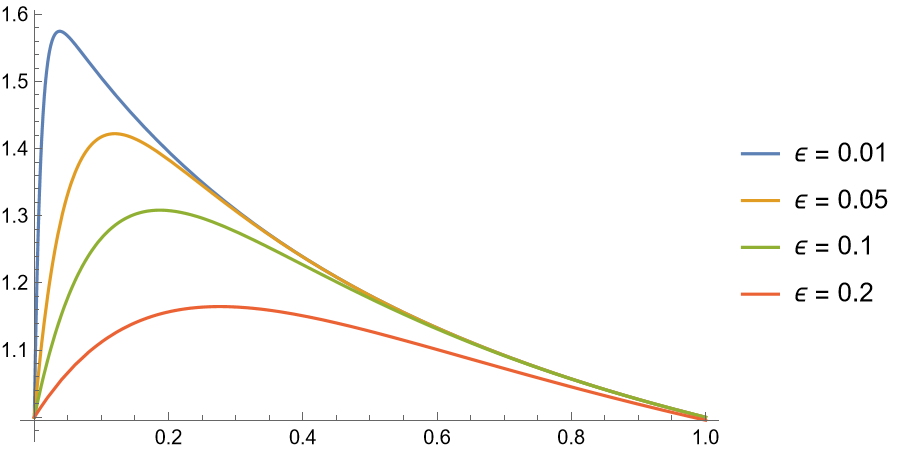
\includegraphics[width=.8\textwidth]{p1.png}
        \end{center}
    
    
    
    \end{enumerate}
\end{solution}

%----------------------------------------------------------------------------------------------------%
%\vskip 20pt
\newpage

%---------------%
%---Problem 2---%
%---------------%

%--status--$

\begin{problem}
    Consider the singular equation
    \[
        \eps y'' - x^2y' - y = 0,   
    \]
    with $y(0) = y(1) = 1$ and with $0 < \eps \ll 1.$
    \begin{enumerate}
        \item [(a)] With the method of dominant balance, show that there are three distinguished limits: $\xi = \eps^{1/2}, \xi = \eps, \xi = 1$ (the outer problem). Write down each of the problems in the various distinguished limits.
        \item [(b)] Obtain the leading order uniform approximation (hint: there are boundary layers at $x=0$ and $x=1$.)
        \item [(c)] Plot the uniform solution for $\eps = 0.01,0.05,0.1,0.2.$
    \end{enumerate}
\end{problem}

\begin{solution}
    
    \noindent
    Consider the equation
    \[ 
        \eps y'' - x^2 y' - y = 0,
    \]
    with $y(0) = y(1) = 1$ and with $0 < \eps \ll 1.$
\begin{enumerate}
    \item [(a)] 
    First we wish to use the method of dominant balance to find the three distinguished limits. Notice that this is a singular problem since $\eps$ is in front of the highest derivative. Furthermore, $b(x) = -x^2$ and $c(x) = - 1$. As $b(x) < 0$ everywhere except at zero, we expect boundary layers at $x = 1$ and $x = 0$ since $b(0) = 0$. 

    \noindent
    First let's consider the distinguished limit near $x=0$. Consider the stretched variable
    \[ 
        \xi = \frac{x}{\delta}.
    \] 
    The change of variable gives the chain rule
    \begin{align*}
        y_x &= y_\xi \xi_x = \frac{1}{\delta}y_\xi,\\
        y_{xx} &= \frac{1}{\delta^2}y_{\xi \xi}. 
    \end{align*}
    Plugging these in and multiplying through by $\delta^2$ yields
    \[ 
        \eps y_{\xi\xi} + \delta^3 \xi^2 y_{\xi} - \delta^2 y = 0.
    \]
    Dropping the smallest term (the second) gives the dominant balance as
    \[ 
        \eps y_{\xi \xi} - \delta^2 y = 0.
    \]
    To balance this we require
    \[ 
        \delta = \eps^{1/2}.
    \]
    Therefore there is a boundary layer at $x = 0$ which has characteristic width $\O(\eps^{1/2}).$

    \noindent
    Next let's study the distinguished limit near $x = 1$ with the stretched variable 
    \[ 
        \xi = \frac{1 - x}{\delta}.
    \]
    The change of variable gives the chain rule
    \begin{align*}
        y_x &= -\frac{1}{\delta}y_{\xi},\\
        y_{xx} &= \frac{1}{\delta^2}y_{\xi \xi}.
    \end{align*}
    Plugging these in and multiplying through by $\delta^2$ yields
    \[ 
        \eps y_{\xi \xi} - \delta(\delta\xi - 1)^2y_\xi - \delta^2 y = 0.
    \]
    Dropping the smallest terms gives the leading order equation
    \[ 
        \eps y_{\xi \xi} + \delta y_{\xi} = 0.
    \]
    to balance this we require
    \[ 
        \delta = \eps.
    \]
    Therefore there is a boundary layer at $x = 1$ with characteristic width $\O(\eps)$. 
    


    \item [(b)]
    
    \noindent
    {\it Outer Solution} - the outer solution is given by plugging the expansion
    \[ 
        y = y_0 + \eps y_1 + \cdots,
    \]
    into the governing equation yields the leading order equation
    \[ 
        -x^2y_{0_x} - y_0 = 0,
    \]    
    whose solution is
    \[ 
        y_0 = C e^{1/x} = y_{\text{out}}.
    \]


    \noindent
    {\it Inner Solution} - There are two boundary layers for the inner problem. Let's first consider the inner solution near $x = 0$ with $\xi = x/\eps^{1/2}$ which has a dominant solution 
    \[ 
        y_{\xi \xi} - y = 0.
    \] 
    Using the expansion
    \[ 
        y = y_0 + \eps y_1 + \cdots,
    \]
    We get the leading order solution to be
    \[ 
        y_{0_{\xi\xi}} - y_0 = 0,
    \]
    which has the solution
    \[ 
        Ae^{-\xi} + Be^{\xi} = 0.
    \]
    For matching, we require our solution to be bounded and thus we set $B = 0$ and applying the boundary condition $y_0(0) = 1$ gives the leading order solution
    \[ 
        y_0(\xi) = e^{-\xi} = y_{\text{in (left)}}.
    \]
    Next let's consider the inner solution near $x=1$ with $\xi = (1-x)/\eps$ which has a dominant solution of
    \[ 
        y_{\xi \xi} - y_{\xi} = 0.
    \]
    Using the expansion
    \[ 
        y = y_0 + \eps y_1 + \cdots,
    \]
    We get the leading order solution to be
    \[ 
        y_{0_{\xi\xi}} + y_{0_\xi} = 0,
    \]
    which has the solution
    \[ 
        y_0 = Ae^{-\xi} + (1-A) = y_{\text{in (right)}}.
    \]

    \noindent
    {\it Matching} - Now we must match our solutions on the left and right. Let's first consider $x = 0$ which gives us
    \begin{align*}
        \lim_{x \to 0} u_{\text{out}} &= \lim_{x \to \infty} u_{\text{in(left)}}\\
        \lim_{x \to 0} C e^{1/x} &= \lim_{x \to \infty} e^{- x/\eps^{1/2}},
    \end{align*}
    and to bound the solution of the outer, we require $C=0$. Thus $u_{\text{out}} = 0$. Next we match the solution near $x = 1$ and thus
    \begin{align*}
        \lim_{x \to 1} u_{\text{out}} &= \lim_{x \to \infty} u_{\text{in(right)}}\\
        0 &=  \lim_{x \to \infty} Ae^{-\xi} + (1-A),
    \end{align*}
    which is only true if $A=1$. The uniform solution is of the form
    \begin{align*}
        u &= u_{\text{out}} + u_{\text{in (left)}} + u_{\text{in (right)}} - u_{\text{match (left)}} - u_{\text{match (left)}}\\
        u &= 0 + e^{-\frac{x}{\eps^{1/2}}} + e^{-\frac{1-x}{\eps}} - 0\\
        u &= \text{exp}\paren{-\frac{x}{\eps^{1/2}}} + \text{exp}\paren{-\frac{1-x}{\eps}}.
    \end{align*}
    
    \item[(c)]
    Using Mathematica we can plot the uniform solution for $\eps = 0.01,0.05,0.1,0.2$ which gives the following figure.
    \begin{center}
        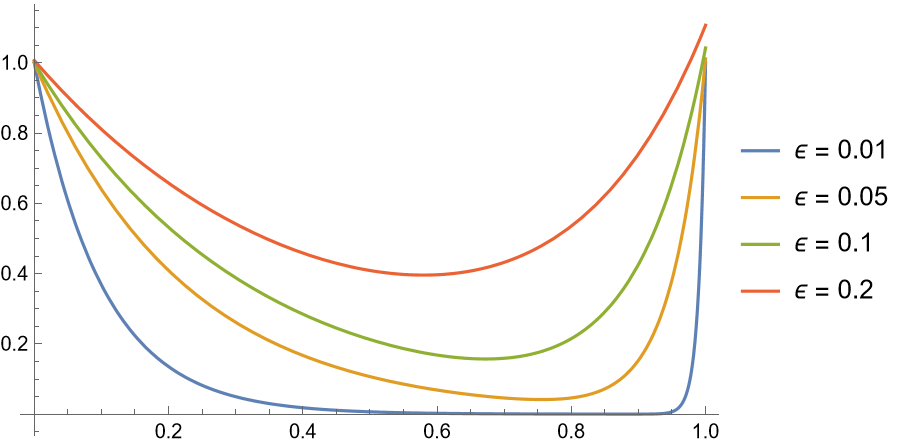
\includegraphics[width=.8\textwidth]{p2.png}
    \end{center}
\end{enumerate}
\end{solution}

%----------------------------------------------------------------------------------------------------%
%\vskip 20pt
\newpage

\end{document}